\documentclass[margin,line]{resume}
\usepackage[hidelinks]{hyperref}
\usepackage{tikz}
\usepackage{enumitem}
\usepackage{fontawesome5}
\setlength{\textheight}{9.7in}

\begin{document}
\begin{tikzpicture}
\clip (0,0) circle (1cm) ;
\node[anchor=center] at (0,0) {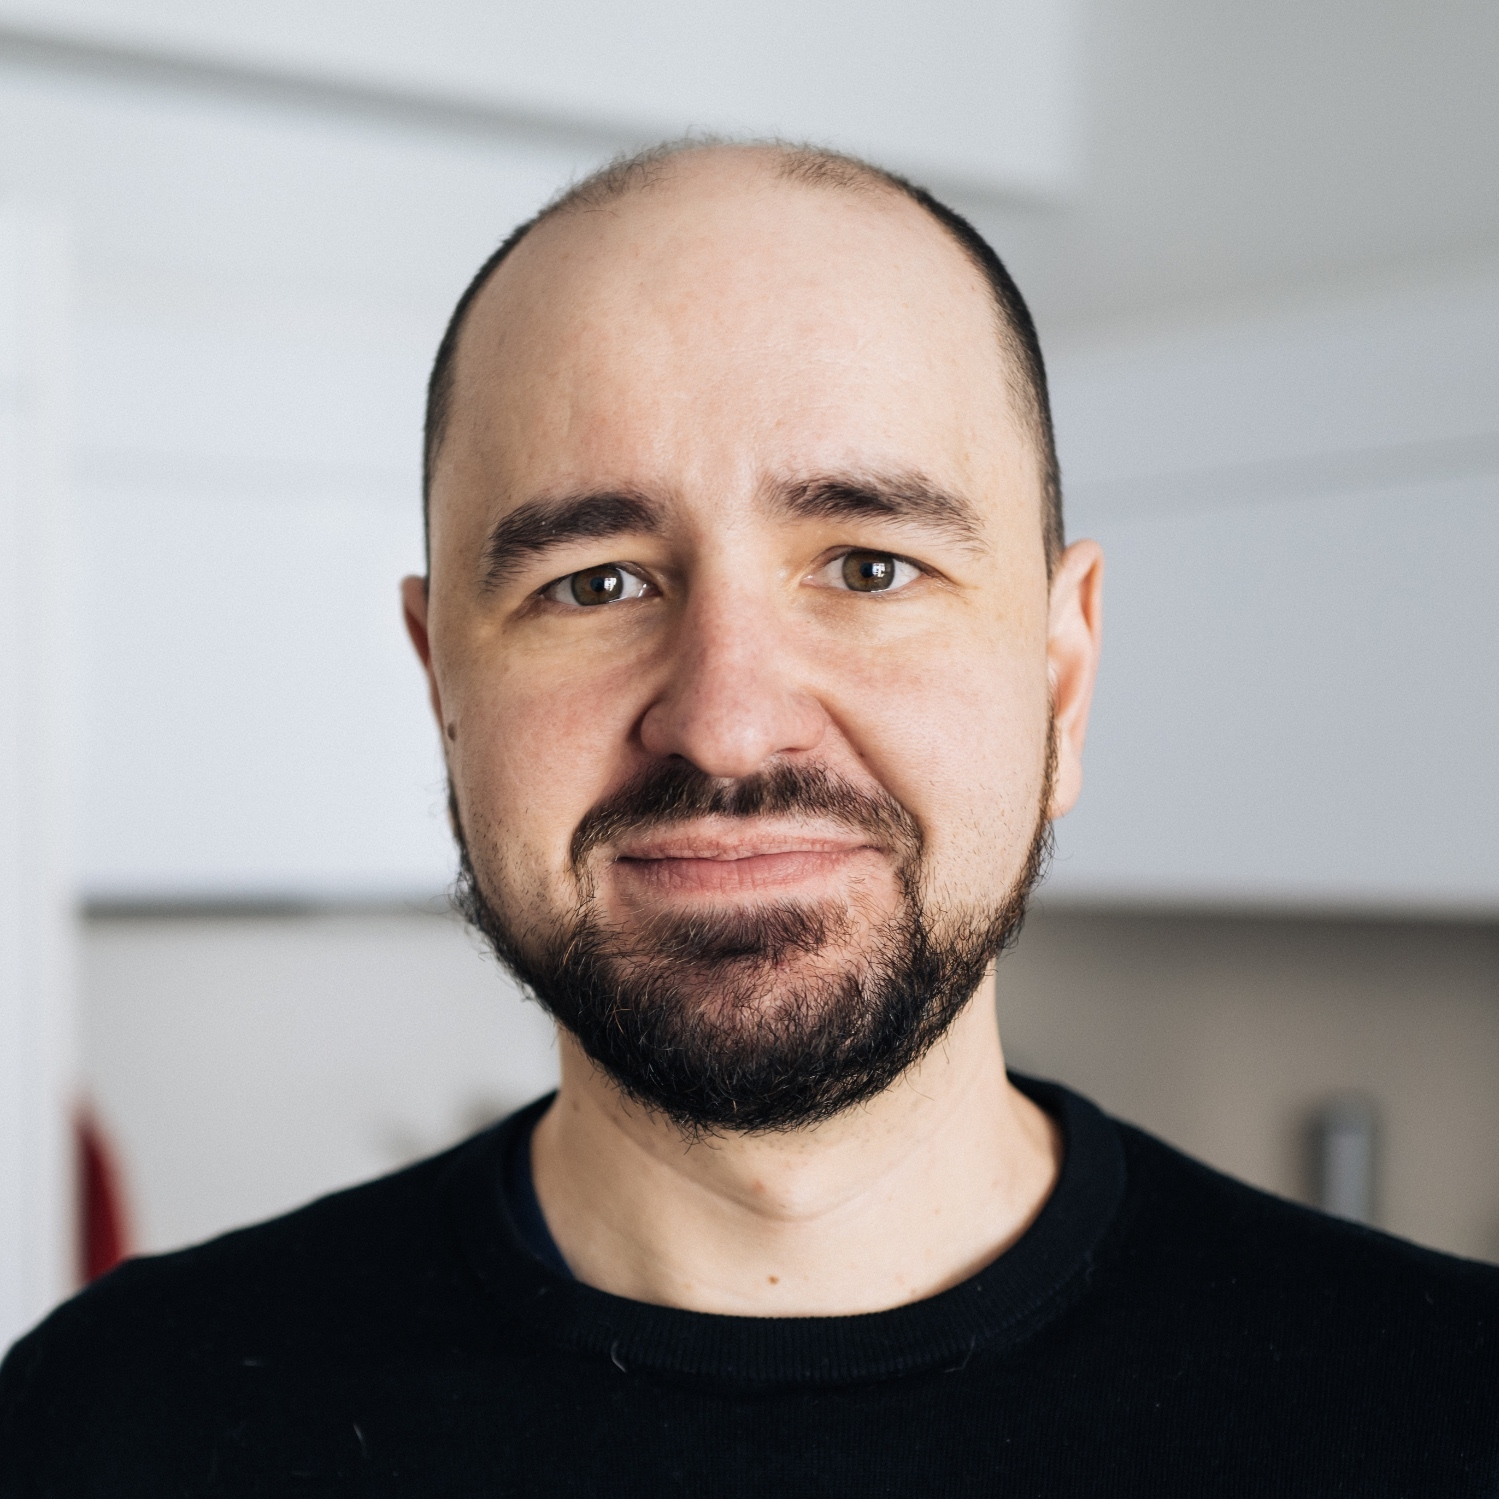
\includegraphics[width=2cm]{myface}};
\end{tikzpicture} \name{\Large Brenden Matthews}
\begin{resume}

\section{Contact}
\begin{tabular}{@{}l|l@{}}
 \href{mailto:brenden@brndn.io}{\faEnvelope\ brenden@brndn.io} & \href{https://github.com/brndnmtthws}{\faGithub\ github.com/brndnmtthws} \\
 \href{https://brndn.io}{\faBlog\ brndn.io} & \href{https://linkedin.com/in/brndnmtthws}{\faLinkedin\ linkedin.com/in/brndnmtthws}
\end{tabular}

\vspace{10pt}

\section{Professional Summary}

Accomplished software engineer with extensive experience in many programming languages and large-scale infrastructure. Published author of two Rust books and creator of multiple open-source projects with 10k+ combined GitHub stars. Skilled in architecting high-performance, highly available systems, mentoring cross-functional teams, and driving technical excellence across organizations.

\begin{itemize}
    \item Founded and scaled multiple businesses, providing full-stack solutions and overseeing end-to-end product development.
    \item Authored two best-selling Rust programming books, establishing recognized expertise and community engagement.
    \item Advised global clients on cloud migrations and Kubernetes-based solutions, boosting reliability while cutting operational costs.
    \item Developed a Rust-based online coding curriculum, mentoring 1,000+ students and generating additional revenue streams.
    \item Delivered keynote speeches at major tech conferences, sharing insights on Rust, cloud computing, and distributed systems.
    \item Built multiple high-impact open-source projects:
        \begin{itemize}
            \item \href{https://github.com/brndnmtthws/conky/}{\textbf{Conky}} (7.4k+ stars): A cross-platform system monitor with extensive customization.
            \item \href{https://github.com/brndnmtthws/thetagang/}{\textbf{ThetaGang}} (2.1k+ stars): Equity options trading platform leveraging advanced data processing.
            \item \href{https://github.com/brndnmtthws/dryoc/}{\textbf{dryoc}} (290+ stars): A Rust cryptographic library offering memory-safe APIs.
        \end{itemize}
\end{itemize}

\vspace{10pt}

\section{Technical Skills}

\begin{itemize}
    \item \textbf{Languages}: Rust, C, C++, Python, JavaScript, TypeScript, Go, Java, Scala, Clojure, Ruby, Elixir, Erlang, Bash
    \item \textbf{Cloud/Infrastructure}: Kubernetes, Docker, Mesos, Nomad, Terraform, AWS, GCP, Azure
    \item \textbf{Data Systems}: Kafka, Cassandra, Snowflake, PostgreSQL, ElasticSearch, Spark, RDS, Redshift, Redis, Hadoop, Presto/Athena
    \item \textbf{Tools/Libraries}: PyTorch, TensorFlow, Helm, Prometheus, Grafana, Git, Jenkins, CircleCI
    \item \textbf{Methodologies}: Agile Development, Cross-Functional Roadmapping, DevOps, CI/CD
\end{itemize}

\vspace{10pt}

\section{Professional Experience}

\filbreak
\textbf{owl.co} \hfill \textit{2022 -- 2023}\\
\textit{Software Engineer, New York, NY}

\begin{itemize}
    \item Mentored junior developers and improved development processes under the guidance of the CTO.
    \item Modernized methods for agile development to increase code quality and efficiency.
    \item Lead an effort to 
\end{itemize}

\filbreak
\textbf{Braze, Inc.} \hfill \textit{2018 -- 2019}\\
\textit{Software Engineer, New York, NY}

\begin{itemize}
    \item Orchestrated a large-scale migration from custom deployment scripts to Kubernetes, accelerating feature releases by 30\%.
    \item Deployed Helm and Terraform to automate provisioned environments, cutting manual configuration errors by 50\%.
    \item Built robust CI/CD pipelines to increase deployment reliability by 40\% and reduce lead time for change.
    \item Instituted a unified monitoring strategy (DataDog), issuing proactive alerts and achieving 99.9\% service uptime.
\end{itemize}

\filbreak
\textbf{Citadel LLC} \hfill \textit{2017 -- 2018}\\
\textit{Software Engineer, New York, NY}

\begin{itemize}
    \item Modernized on-prem data infrastructure by integrating AWS and GCP services, lowering time to provision new analytics by 70\%.
    \item Led migration to PostgreSQL and Spark-based architectures, improving query performance by 60\%.
    \item Streamlined large-scale ML model deployment processes, enabling faster experimentation and reduced runtime costs.
\end{itemize}

\filbreak
\textbf{D2IQ (fka Mesosphere)} \hfill \textit{2015 -- 2017}\\
\textit{Software Engineer \& Sales Engineering Lead, San Francisco, CA}

\begin{itemize}
    \item Assembled the first sales engineering team, bridging technical and business domains to close multi-million-dollar accounts.
    \item Guided Fortune 500 firms in containerization and distributed systems adoption, accelerating cloud-native transformation.
    \item Contributed to frameworks like Hadoop, Chronos, Marathon, and marathon-lb, enabling mission-critical workloads on DC/OS.
\end{itemize}

\filbreak
\textbf{Airbnb, Inc.} \hfill \textit{2013 -- 2015}\\
\textit{Software Engineer, Data Infrastructure, San Francisco, CA}

\begin{itemize}
    \item Built scalable data pipelines using Apache Spark, Hadoop, and Mesos, providing near-real-time analytics across teams.
    \item Contributed to \textbf{Apache Superset} and \textbf{Apache Airflow}, increasing organizational visibility into ETL processes.
    \item Decreased data inconsistency by 90\% with automated verification systems, boosting overall data reliability.
    \item Optimized critical data retrieval mechanisms, achieving a 100x reduction in query times.
\end{itemize}

\filbreak
\textbf{Newfield Wireless, Inc.} \hfill \textit{2009 -- 2012}\\
\textit{Senior Software Engineer, Berkeley, CA}

\begin{itemize}
    \item Developed real-time LTE network parsing tools, improving system throughput and cutting analysis time by 50\%.
    \item Built custom database solutions with integrated query capabilities for instant investigation of streaming metrics.
    \item Expanded high-performance data pipelines in C++ and Python, enabling rapid troubleshooting for telecom operators.
\end{itemize}

\filbreak
\textbf{Real Time Measurements, Inc.} \hfill \textit{2003 -- 2009}\\
\textit{Software Engineer, Calgary, AB}

\begin{itemize}
    \item Created embedded software for industrial hardware, focusing on real-time reliability and performance optimization.
    \item Developed web services for remote device control, cutting manual intervention by 80\%.
    \item Reduced IT overhead by automating server provisioning and configuration.
\end{itemize}

\vspace{10pt}

\section{Open Source Contributions}

\begin{itemize}
    \item Contributed to major Apache projects: Kafka, Superset, Airflow, Spark, and Mesos (PMC member).
    \item Maintained tools collectively earning 10k+ GitHub stars, reflecting wide community adoption.
\end{itemize}

\vspace{10pt}

\section{Published Works}

\begin{itemize}
    \item \href{https://www.manning.com/books/code-like-a-pro-in-rust}{\textit{Code Like a Pro in Rust}} (Manning Publications) \hfill ISBN: 9781617299643
    \item \href{https://www.manning.com/books/idiomatic-rust}{\textit{Idiomatic Rust: Code Like a Rustacean}} (Manning Publications) \hfill ISBN: 9781633437463
\end{itemize}

\vspace{10pt}

\section{Public Speaking}

\begin{itemize}
    \item Presented at \textbf{All Things Open}, \textbf{QCon}, \textbf{MesosCon}, \textbf{Spark Summit}, \textbf{LinuxCon}, highlighting best practices for Rust and cloud computing.
    \item Keynoted on distributed systems and DevOps, offering insights on scalable architectures to global audiences.
\end{itemize}

\end{resume}
\end{document}
